%%=====================================================================================
%%
%%       Filename:  Assignment2_Solution.tex
%%
%%    Description:  Solution to problem 2.
%%
%%        Version:  1.0
%%        Created:  02/25/2017
%%       Revision:  none
%%
%%         Author:  Dilawar Singh (), dilawars@ncbs.res.in
%%   Organization:  NCBS Bangalore
%%      Copyright:  Copyright (c) 2017, Dilawar Singh
%%
%%          Notes:  
%%                
%%=====================================================================================

\documentclass[a4paper,10pt]{article}
\usepackage{pgf,tikz}
\usepackage{amsmath}
\usepackage{amssymb}
\usepackage{grffile}
\usetikzlibrary{shapes,backgrounds,decorations,decorations.pathmorphing}
\usetikzlibrary{calc,positioning}

% Title Page
\title{Solution to Assignment 2} 
\author{Dilawar Singh}
%\usepackage{ebgaramond}
\usepackage{palatino}
\usepackage[sfdefault,light]{FiraSans}
\ifluatex
\else
\usepackage[T1]{fontenc}
\fi
\date{\today}

\begin{document}
\maketitle

Let me start with solutions from assignment submission. 

\section{Drawing without replacement} 

We have a jar with $N$ balls, out of which $b$ are blue and rest are red. I draw
a ball at random but do not put it back.  Clearly it is not a Markovian process
since at each step the probability of drawing red (or blue) ball is changing. At
time zero, probability of drawing a blue ball is $\frac{b}{N}$ which changes to
either $\frac{b-1}{N-1}$ if drew blue ball or $\frac{b}{N-1}$ if I drew red ball
now. I can define states in the process.  Let say they are {\tt BLUE\_DRAWN} and
{\tt RED\_DRAWN}. The transition graph of this process will look like the
following.

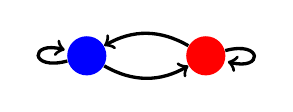
\begin{tikzpicture}[scale=1, every node/.style={circle}, inner sep=5pt ]
    \node[fill=blue] (blue) {};
    \node[fill=red, right=of blue] (red)  {};
    \draw[very thick,->] (blue) to[bend right] (red);
    \draw[very thick,->] (red) to[bend right] (blue);
    \draw[very thick,->] (red) edge[loop right] (red);
    \draw[very thick,->] (blue) edge[loop left] (blue);
    
\end{tikzpicture}    

Where arrow in graph shows the transition to head state given system is in tail
state now. For example, \tikz{ \node[fill=red,circle] (red) {};
\node[fill=blue,circle,right=of red ] (blue) {}; \draw[->] (red) -- node[above]
{$p$} (blue) } depicts the process of drawing blue ball given that red was drawn
just before. The number on arrow $p$ is the probability of this transition. I
leave it upto you to write the transition matrix for this system using these two
states and convince yourself that this is not Markovian.

A couple of attempts were made to turn it into a Markovian by introducing more
states: a {\tt NULL\_BLUE} \tikz \node[circle,fill=blue!50] {}; and {\tt
NULL\_RED} \tikz \node[circle,fill=red!50] {}; states. 

The state transition graph is following.

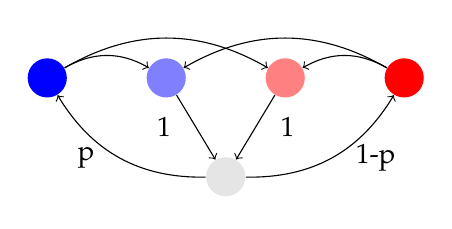
\begin{tikzpicture}[scale=1, every node/.style={circle}, inner sep=5pt ]
    \node[fill=blue] (blue) {};
    \node[fill=blue!50,right=of blue] (nullblue) {};
    \node[fill=red!50, right=of nullblue] (nullred)  {};
    \node[fill=red, right=of nullred] (red)  {};
    \node[fill=black!10,below=of $(nullblue)!0.5!(nullred)$] (null) {};

    \draw[->] (blue) to[bend left] (nullred);
    \draw[->] (blue) to[bend left] (nullblue);

    \draw[->] (red) to[bend right] (nullred);
    \draw[->] (red) to[bend right] (nullblue);

    \draw[->] (nullred) to node[midway,right] {1} (null);
    \draw[->] (nullblue) to node[midway,left] {1} (null);

    \draw[->] (null) to[bend left] node[midway,left] {p} (blue);
    \draw[->] (null) to[bend right] node[midway,right] {1-p} (red);
    
\end{tikzpicture}    

The state transition graph still does not have constant probabilities. In
short, I could not turn this non-Markovian process to Markovian. However, if
someone has come so far, I've given them full credit. If you know a way to
convert this to Markovian process, let me know.

\section{By \emph{merging} states}

%In this approach, you already start with a process which is Markovian and merge
%states together till it becomes a non-Markovian. Then you present it in reverse
%to your TA.

A solution is given in submissions as following. Consider you are playing the
game of "snake and ladder".  You consider the position of player on the board
coarsely. You note down the row (e.g. row 1, 2, etc.) rather than cell (2x1,
9x4, etc.). The claim is that this stochastic process sampled coarsely is not a
Markovian process because \emph{transition from row $i$ to row $j$ is dependant
on previous transition $x \rightarrow i$ }. 

The idea is correct and has been awarded full marks. However 'snake and ladder'
seen coarsely as row to row transition may still be Markovian. If merging some
states of a Markovian process still leads to a Markovian process, such processes
are callled \emph{lumpable} [Kemeny and Snell, 1976; Peng 1996]. Lumping is
computationally expensive process.

Simulation of 'snake and ladder' game suggest that coarse level description may
still be Markovian for N games (where N > 4 ). The transition probabilities
matrix does not change whether we describe the process at the level of cells or
at the level of rows.

\subsection{Simulation of game}

I simulated a game of snake and ladder 10000 times and
computed the transition probabilities; first by taking cell level view and
second by taking coarse cell level view.

\begin{figure}[ht!]
\begin{center}
    \includegraphics[width=1\textwidth]{./snake_and_ladder.py.png}
\end{center}
\caption{Subplot 1 shows the transition probabilities of cell to cell
    transitions after 20 games. Subplot 2 shows the transitions probabilities of
    row to row transitions after 20 games. Both of these do not change after
roughly 3 games (shown in subplot 3) }
\label{fig:}
\end{figure}

\section{Non Markovian Neuron}

Let assume that we are watching a neuron every 1 ms. We note down $\uparrow$
when the neuron fires and $\_$ otherwise. We notice that probability of neuron
firing is roughly $p$. We also know that if a neuron just has fired, then it can
not fire for next 2 ms (2 steps) (neuron's \textbf{refactory period}).  As long
as we are describing this process using two states $\uparrow$ and $\_$, it is
not Markovian since probability of neuron firing is dependant on weather it has
fired in previous two steps or not.

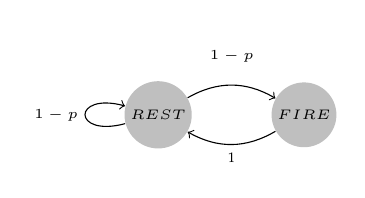
\begin{tikzpicture}[scale=1 , every node/.style={circle,fill=gray!50 } ]
    \tiny
    \node[ ] (resting) {$REST$};
    \node[right=of resting ] (fire) {$FIRE$};
    \draw[->] (resting) to[loop left] node[fill=none] {$1-p$} (resting);
    \draw[->] (resting) to[above,bend left] node[fill=none] {$1-p$} (fire);
    \draw[->] (fire) to[below,bend left] node[fill=none] {1} (resting);
\end{tikzpicture}    

Above transition graph represents a Markovian process and can handle refactory
period of 1 step (how?). Many single neuron spike trains can be represented by
such a simple system.

To make it Markovian when refactory period is longer than 1 step, we introduce
two more state variables $FIRE{-1}$ and $FIRE{-2}$. The transition diagram is
following. Write down the transition matrix and convince yourself that it is a
Markov.

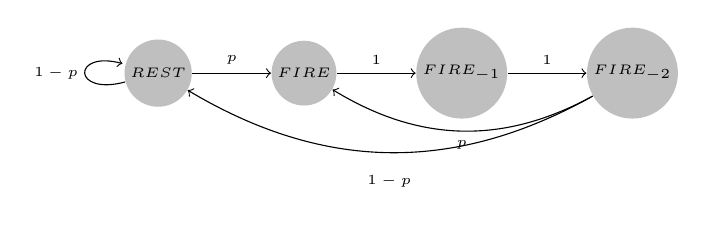
\begin{tikzpicture}[scale=1 , every node/.style={circle,fill=gray!50 } ]
    \tiny
    \node[ ] (resting) {$REST$};
    \node[right=of resting ] (fire) {$FIRE$};
    \node[right=of fire ] (fireprev) {$FIRE_{-1}$};
    \node[right=of fireprev ] (fireprevprev) {$FIRE_{-2}$};

    \draw[->] (resting) edge[above,midway] node[draw=none,fill=none] {$p$} (fire);
    \draw[->] (resting) edge[loop left] node[draw=none,fill=none] {$1-p$} (resting);
    \draw[->] (fire) edge[above,midway] node[draw=none,fill=none] {$1$} (fireprev);
    \draw[->] (fireprev) edge[above,midway] node[draw=none,fill=none] {$1$} (fireprevprev);
    \draw[->] (fireprevprev) edge[bend left,below,midway]
                    node[draw=none,fill=none] {$p$} (fire);
    \draw[->] (fireprevprev) edge[bend left,below,midway]
                    node[draw=none,fill=none] {$1-p$} (resting);
    
\end{tikzpicture}    

Its easy to see that state $FIRE_2$ and state $REST$ can be merged together and
matrix is still Markov. This is trivial case of lumpability.


\end{document}          

